\documentclass{article}
\usepackage[utf8]{inputenc}
\usepackage[english]{babel}
\usepackage{amsmath}
\usepackage{amssymb}
\usepackage{physics}
\usepackage{nicefrac}
\usepackage{graphics}
\usepackage{graphicx}
\usepackage{subfig}
\usepackage{svg}
\usepackage{pdfpages}
\usepackage{placeins}
\usepackage[a4paper, top=2cm, bottom=2.5cm, left=3cm, right=3cm]{geometry}
\usepackage[colorlinks=true, urlcolor=blue, linkcolor=blue]{hyperref}
\usepackage{siunitx}
\sisetup{
	locale = UK,
	per-mode = fraction,    
	separate-uncertainty
}
\usepackage{comment}
\usepackage{float}

\newcommand{\namen}{Fabian Ganzer}
\newcommand{\headline}{IST research project: \\Neglection of matrix elements in coupling matrix of Ising model for active user detection}

\hypersetup{pdfauthor=\namen, pdftitle=\headline}

\title{\headline}
\author{\namen }

\date{\begin{tabular}{ll}
		Time period:  & winter semester 2024/2025         \\
		Location:      & INSA Lyon, CITI laboratory          \\
		Supervisors: &  Prof. Claire Goursaud, Romain Piron	          \\
\end{tabular}}


\begin{document}
	\maketitle 
	\tableofcontents
	\newpage
	\section{Hamming distance}
	The goal of the annealing process is to recover the activity pattern. Due to the modification of the coupling matrix, one introduces errors in the problem leading to bit errors in the activity pattern. How strong the deviation of the determined activity pattern from the actual activity pattern is, can be quantified using the hamming distance $d_\text{H}$.
	\begin{figure}[h]
		\centering
		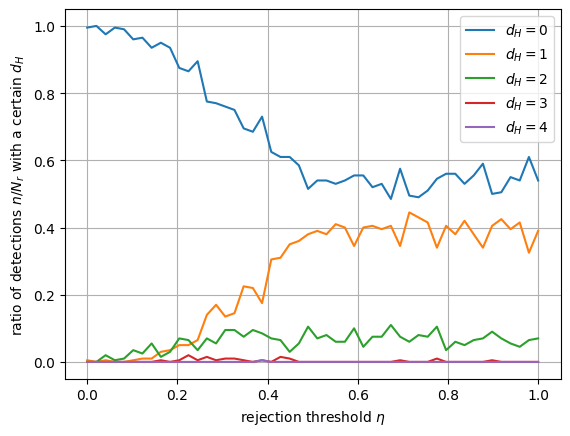
\includegraphics[width=0.75\textwidth]{img/hamming_rule_1.png}
		\caption{ratio of correct detections for different hamming distances}
		\label{fig:hamming rule 1}
	\end{figure}

	\begin{figure}[h]
		\centering
		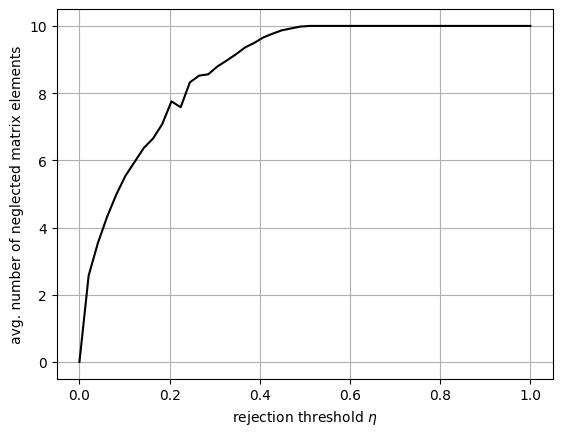
\includegraphics[width=0.75\textwidth]{img/N_neglected_rule_1.png}
		\caption{average number of neglected matrix elements}
		\label{fig:N neglected rule 1}
	\end{figure}

	\begin{figure}[h]
		\centering
		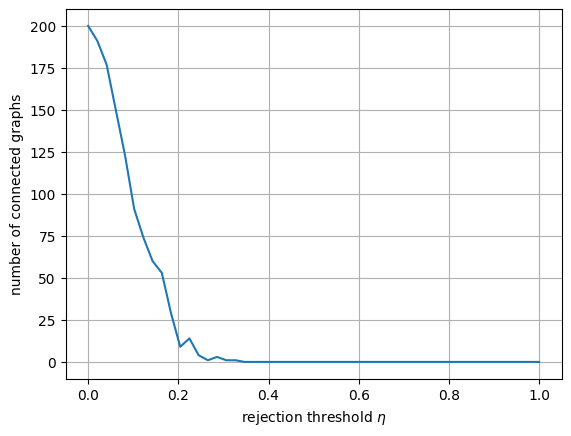
\includegraphics[width=0.75\textwidth]{img/N_connected_rule_1.png}
		\caption{average number of connected graphs}
		\label{fig:N }
	\end{figure}
	
	\section{Comparison with a conventional correlation receiver (CCR)}
	
	\section{Dependence on the degree of the nodes}
	Now, it shall be examined, whether the correctness of the detection correlates with the degree of the nodes of the graph.  To do so, many instances of the problem are generated and for each instance, the maximum, minimum and average degree over all nodes in the graph are determined. It is counted, how many detections are correct. The following diagrams are generated for a neglection threshold of 0.08.
	
	\begin{figure}[h]
		\subfloat[min. degree]{
			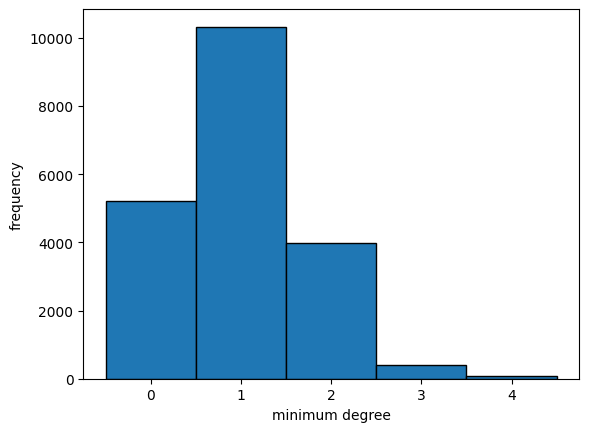
\includegraphics[width=0.33\textwidth]{img/deg_min.png}
		}
		\subfloat[avg. degree]{
			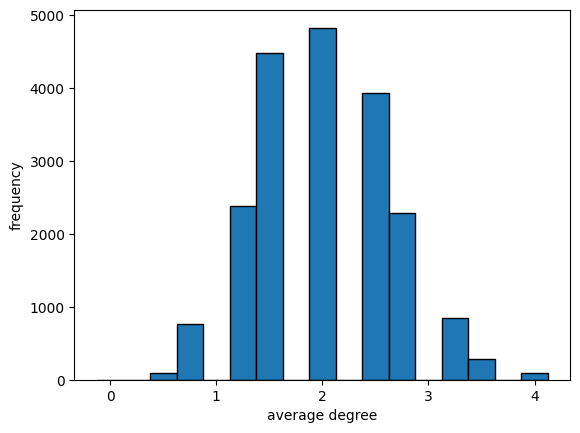
\includegraphics[width=0.33\textwidth]{img/deg_avg.png}
		}
		\subfloat[max. degree]{
			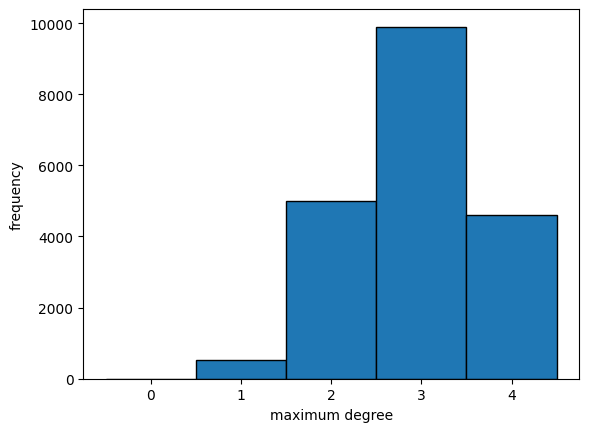
\includegraphics[width=0.33\textwidth]{img/deg_max.png}
		}
	\caption{distribution of graph counts with respect to different degrees}
	\label{fig:degrees}
	\end{figure}
	The purpose of the diagrams in Fig.~\ref{fig:degrees} is to verify how many values will be taken into consideration for each degree in order to correctly understand the following diagrams. For instance, for a {\tt neglection\_thres} of 0.08, and neglection rule 1 (threshold method), one can see that the distribution of the graph occurrences with respect to the maximum degree is approx. centered around 3, meaning that the following evaluation of correct results should yield the highest accuracy for 3 in the max. degree diagram.
	Looking at the avg. degree distribution, one notices, that there are certain average degrees which don't occur a single time. This is because they are forbidden by the topology of the graph. For instance, if $N=5$, an average degree of 1 is impossible because if there are two edges in the graph, the average degree will be $\nicefrac{4}{5}$ and if there are three edges in the graph, the avg. degree will be $\nicefrac{6}{5}$ but there will be nothing in between. 
	
	\begin{figure}[h]
		\centering
		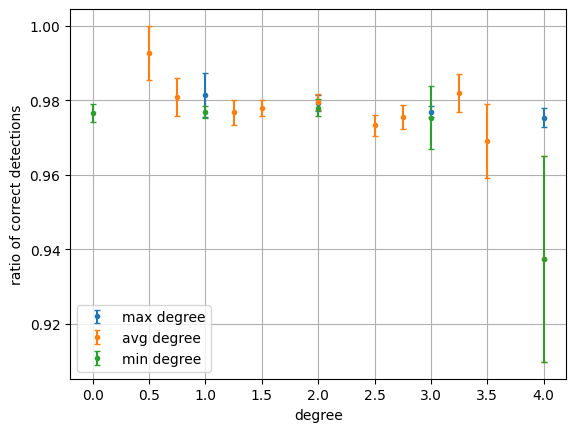
\includegraphics[width=0.75\textwidth]{img/deg_ratio.png}
		\caption{evolution of correctness ratio with respect to the degree of the nodes}
		\label{fig:correctness degree}
	\end{figure}
	The results can be seen in Fig.~\ref{fig:correctness degree}. It can be observed that the ratio of correct detections remains relatively high in the regime of over 92\,\%. For each category (min/avg/max degree) there seems to be a very slight decrease of the ratio of correct detections with increasing degree. This is counterintuitive since one would expect the correctness to increase if one allows more couplings because then there are more interactions among the qubits and the interactions in the end are what is expected to increase the correctness of the results. This effect will in the following section be observed again and an interpretation is given there. 
	
	Another observation is, that the error margins vary. For instance, considering the data points for the minimum degree, one can see that for a minimum degree of 1, the margin is the smallest while for a minimum degree of 4, the margin becomes very large. This is because of the size of the underlying data sets. As can be seen in Fig.~\ref{fig:degrees}, there are only very few generations for a minimum degree of 4 while for a minimum degree of 1, the number of generated graphs is maximal. Thus, it is evident, that the accuracy varies accordingly.   
	
	\section{Dependence on the connectedness of the graph}
	A graph is connected, if every node of the graph is connected to at least one other node of the graph. If a graph is not connected, there are at least two subgraphs of qubits not interacting with each other. One might imagine that this yields worse results than a graph describing a situation where every qubit takes part in the interaction. To test this hypothesis, many instances of problems are generated and the ground state is evaluated. For each instance it is determined, if the corresponding graph is connected or not and the evolution of the ratio of correct detections is traced. 
	
	\begin{figure}[h]
		\centering
		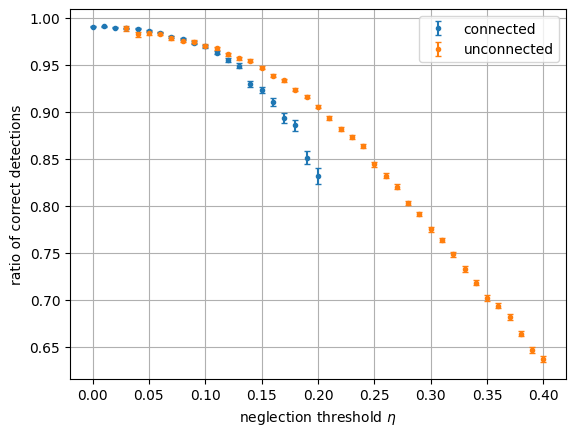
\includegraphics[width=0.75\textwidth]{img/connected_unconnected_rule_1.png}
		\caption{dependence of correct detections on the threshold for connected and unconnected graphs for the threshold method}
		\label{fig:connected unconnected rule 1}
	\end{figure}
	This ratio can be seen in Fig.~\ref{fig:connected unconnected rule 1}. As the rejection threshold increases, the ratio of correct detections drops as expected. What however is surprising, is that for larger rejection thresholds, the ratio of correct detections is dropping faster for connected graphs than for non-connected graphs. We suspect this is not because the property of having a connected graph leads to worse results but rather that the connectedness is a measure of how difficult the problem we are trying to solve really is. In other words, we achieve a lower ratio of correct solutions for connected graphs because the AUD problems that correspond to connected graphs are more difficult to solve than those corresponding to non-connected graphs. This is plausible, because a coupling is computed as $J_{ij} = -\frac{1}{2}|\vec p_i^\dagger \vec p_j|^2$. This means, if the two pilot sequences $\vec p_i$ are very similar, the corresponding coupling will be large. In a connected graph, enough couplings are at least as large as necessary not to get neglected, which only happens if the pilot sequences are similar. And if the pilot sequences are similar, it es easy to guess one bit wrong. 
	
	Further it can be observed that for $\eta>0.2$, no data points are on the curve for the connected graphs anymore. This is because for those rejection thresholds, it is very unlikely to generate a connected graph as shown in Fig.~\ref{fig:}
	
	 	
	\begin{figure}[h]
		\subfloat[number method]{
			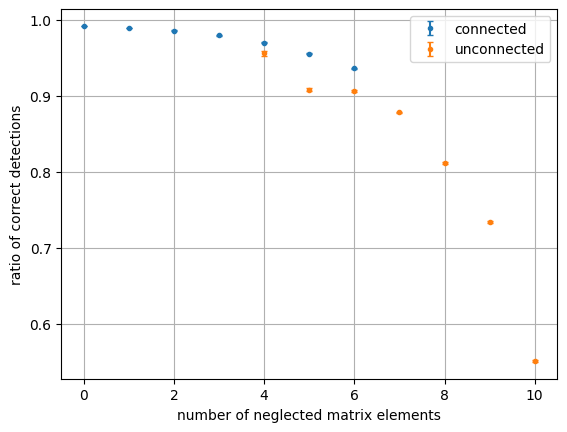
\includegraphics[width=0.49\textwidth]{img/connected_unconnected_rule_2.png}
		}
		\subfloat[max degree method]{
			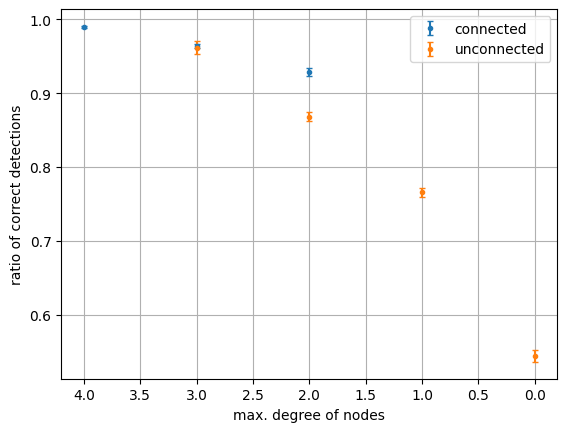
\includegraphics[width=0.49\textwidth]{img/connected_unconnected_rule_3.png}
		}
	\caption{ratio of correct detections for both other methods}
	\label{fig:connected unconnected rule 2 and 3}
	\end{figure}
For rejection rules 2 and 3, the results are shown in Fig.~\ref{fig:connected unconnected rule 2 and 3}. In contrast to the threshold method from Fig.~\ref{fig:connected unconnected rule 1}, the connected graphs seem to yield better results. To explain this observation, an examination and comparison of the coupling matrix in those cases with the coupling matrix for the first case would be necessary. 


	
\end{document}